\section{Einleitung}
\label{sec:intro}
1965 prognostizierte Gordon Moore, dass sich die Anzahl der auf einem Schaltkreis befindlichen Transistoren ca. alle 2 Jahre verdoppeln würde. Bis heute trifft diese Annahme, das sogenannte Moore'sche Gesetz, weitgehend zu. Zunehmend tritt die Frage auf, ob es eine obere Grenze für das Gesetz gibt, denn mit der Anzahl steigt auch die Dichte der Transistoren. Überschreitet diese ein gewisses Maß, entstehen Quanteneffekte und die Hardware verhält sich nicht mehr wie in der klassischen Physik erwartet. Die Beschäftigung mit Quantenmechanik in Bezug auf Computer wird daher immer wichtiger. Einige Firmen wie beispielsweise IBM oder D-Wave stellen bereits Quantum Computer zu einer cloudbasierten Nutzung zur Verfügung. \cite{moore, qc-mainzer}
\\\\
Auch im Bereich der Künstlichen Intelligenz (KI) entwickelt sich immer größer werdendes Interesse. So gab es in der Forschung bereits große Durchbrüche in Bereichen wie der Robotik, Mustererkennung und Spracherkennung. Erste Ideen, Neuronen technisch zu realisieren, entwickelten sich bereits 1943 mit dem McCulloch-Pitts-Neuron. Heute werden komplexe Neuronale Netze (NN) verwendet. Ein Beispiel hierfür ist die sogenannte Boltzmann Machine (BM), die zu den ungerichteten NNs gezählt wird. \cite{ki, Hinton2007}


Es existieren bereits Algorithmen, die auf Grundlage einer Kombination von Quantum Computing und KI arbeiten. Durch den Einsatz von quantenbasierten Berechnungen entstehen Möglichkeiten, welche über die Fähigkeiten einer klassischen KI hinaus gehen. \cite{qc-mainzer}
\\\\
In dieser Arbeit soll eine Methode zur Anomalieerkennung mittels eines hybriden Verfahrens entwickelt und evaluiert werden, bei der ein Quantum Computer als unterstützende Komponente im Lernprozess einer Boltzmann Machine dient. Dafür werden in Kapitel \ref{sec:basics} Grundlagen zum Quantum Computing, Maschinellem Lernen (ML) und Anomalieerkennung eingeführt, Kapitel 3 bietet einen kompakten Überblick über verwandte Arbeiten, Kapitel 4 erläutert die in der Arbeit verwendeten Methoden und Konzepte, wie BMs und einen Ansatz zur Erkennung von Anomalien. Mittels Simulationen und unter Verwendung von Quantum Hardware werden diese in Kapitel 5 evaluiert. Abschließend wird in Kapitel 6 ein Fazit gezogen.

\section{Grundlagen}
\label{sec:basics}
Quantum Computer arbeiten grundlegend anders als klassische Computer, da sie auf anderen physikalischen Gegebenheiten basieren. Daher wird in Abschnitt \ref{subsec:basics-qc} auf Grundbegriffe des Quantum Computings sowie die Unterschiede zwischen dem Quantum Gate Model und Quantum Annealing (QA) eingegangen. In Abschnitt \ref{subsec:basics-ml} werden verschiedene grundlegende Konzepte des ML vorgestellt, da diese Arbeit ein Quantum ML Verfahren verwendet. Da dieses auf ein Problem der Anomalieerkennung angewendet wird, gibt Abschnitt \ref{subsec:basics-ad} eine Einführung in diesen Bereich.

\subsection{Quantum Computing}
\label{subsec:basics-qc}
Berechnungen in klassischen Computern basieren auf Bits, die zu jedem Zeitpunkt entweder den Wert $0$ oder $1$ annehmen können. Mithilfe von Gattern werden diese manipuliert. Quantum Computer hingegen verwenden für Berechnungen Qubits. Der Zustand eines Qubits kann durch folgende Formel dargestellt werden:
\begin{equation}
    \ket{\psi} = \alpha\ket{0} + \beta\ket{1}
\end{equation}
$\alpha$ und $\beta$ geben dabei den Anteil an, zu welchem sich das Qubit im Zustand $0$ bzw. $1$ befindet. Anders als Bits können sich Qubits also in beliebigen Überlagerungszuständen von $0$ und $1$ befinden. Dieses Phänomen wird \emph{Superposition} genannt. Allerdings zerfällt die Überlagerung durch einen Messvorgang und das Qubit landet mit einer Wahrscheinlichkeit von $|\alpha|^2$ in Zustand $0$ und einer Wahrscheinlichkeit von $|\beta|^2$ in Zustand $1$. \cite{qc-homeister}
\\\\
Es gibt zwei Arten des Quantum Computings, das Quantum Gate Model und das Adiabatische Quantum Computing (AQC). Quantum Gate Computer arbeiten ebenso wie klassische Rechner auf Basis von Gattern, mithilfe derer Zustände von Qubits verändert werden können. Die für diese Arbeit relevante Gruppe von Quantum Computern bilden die Quantum Annealer, welche dem AQC zuzuordnen sind. Als Eingabe benötigen sie eine zu minimierende Zielfunktion. Diese wird Hamiltonian genannt und beschreibt die Energie eines physikalischen Systems. Das Ziel eines Quantum Annealers ist es, die Funktion zu minimieren, d.h. den Zustand mit der geringsten Energie zu finden \cite{qc-homeister}. Dabei macht er sich das adiabatische Theorem zunutze. Dieses besagt, dass ein System, welches sich im Grundzustand befindet, im Grundzustand bleibt, solange es langsam genug verändert wird \cite{adiabatic}. Ein Quantum Annealer verwendet daher für den Start seiner Berechnung einen initialen Hamiltonian, bei dem der Grundzustand bekannt ist und versetzt das System, d.h. seine Qubits, in diesen Zustand. Danach wird der initiale Hamiltonian in den finalen Hamiltonian, welcher das Problem kodiert, überführt. Im optimalen, bzw. theoretischen Fall, resultiert das System im Grundzustand des finalen Hamiltonians. Dieser Zustand stellt die optimale Lösung des Problems dar. Die Form des Hamiltonians, der sich während der Berechnung ergibt, kann folgendermaßen dargestellt werden:
\begin{equation}
H(t) = (1 - \frac{t}{T}) * H_{initial} + \frac{t}{T} * H_{final}
\end{equation}
$T$ gibt dabei die Laufzeit des Prozesses an, $t$ den betrachteten Zeitpunkt. Die optimale Lösung kann jedoch nur bei unendlicher Laufzeit und somit nur in der Theorie garantiert werden.
Quantum Annealing zählt daher zu den Heuristiken, einer Gruppe von approximativen Optimierungsverfahren. \cite{qc-homeister, infinite, heuristic}

\subsection{Maschinelles Lernen}
\label{subsec:basics-ml}
Ein Teilgebiet der KI bildet ML. Dieses beschreibt einen Vorgang, der die Erstellung eines Modells anhand von Regeln, die aus Daten abgeleitet werden, beinhaltet. Dies lässt sich \emph{supervised} oder \emph{unsupervised} realisieren. Im supervised Modell sind Klassenlabel bekannt, während im unsupervised Modell Klassenlabel selbst erlernt werden müssen. Eine Möglichkeit, diesen Lernvorgang umzusetzen, bieten NNs. Diese bestehen bildlich gesprochen aus Knoten, den künstlichen Neuronen, und Verbindungen zwischen diesen. Die Funktionsweise eines NNs ist von der Biologie inspiriert. Nervenzellen werden durch elektrische Impulse vorgeschalteter Nervenzellen aktiviert. Im künstlichen Bereich funktioniert dies folgendermaßen.

\begin{figure}[h]
  \centering
  \includegraphics[width=0.5\textwidth]{images/Neuron-weights.pdf}
  \caption{Visualisierung eines künstlichen Neurons mit zwei Eingängen $x_1$ und $x_2$ und einem Ausgang $A$ \cite{ml}}
  \label{fig:nn-weights}
\end{figure}

\noindent Ein künstliches Neuron besitzt Ein- und Ausgänge. Im Beispiel aus Abbildung \ref{fig:nn-weights} gibt es zwei Eingänge $x_1$ und $x_2$ sowie einen Ausgang $A$. Der Eingang eines Neurons entspricht dem Ausgang der jeweils vorgeschalteten Neuronen und kann entweder den Wert $0$ oder $1$ annehmen, je nachdem, ob das Neuron aktiviert wurde ($1$) oder nicht ($0$). Ob ein Neuron aktiviert wird, bestimmt die Summe der gewichteten Eingänge.
Wählt man beispielsweise die Werte $x_1 = 1$, $x_2 = 0$, $w_1 =2$, $w_2 = -1$, ergibt sich als Summe $2\cdot1 - 1\cdot0 = 2$. Übersteigt dieser Wert einen bestimmten Wert, den sogenannten Bias eines Neurons, wird dieses aktiviert, andernfalls verbleibt es im nicht aktivierten Zustand.
\begin{figure}[!h]
  \centering
  \includegraphics[width=0.3\textwidth, angle=-90]{images/NeuronalesNetz.pdf}
  \caption{Schema eines Neuronalen Netzes \cite{ml}}
  \label{fig:nn}
\end{figure}
\\Ein NN entsteht durch das Zusammenschalten mehrerer solcher künstlichen Neuronen. Abbildung \ref{fig:nn} zeigt den schematischen Aufbau eines NNs.
NNs können verschieden viele Ebenen besitzen. Eine Gruppe von NNs, welche aus zwei Ebenen bestehen, bilden Restricted Boltzmann Machines (RBM). \cite{ml, Adachi15}

\subsection{Erkennung von Anomalien}
\label{subsec:basics-ad}
Die Erkennung von Anomalien ist ein ML Prozess, der Datenpunkte, Ereignisse und Beobachtungen identifiziert, welche vom normalen Verhalten eines Datensatzes abweichen. Besonders die Erkennung von Anomalien in Zeitreihendaten ist ein Problem von entscheidender Bedeutung, da hier bösartige Angriffe auf Systeme für industrielle Anwendungen beobachtet werden können. Weiterhin wird Anomalieerkennung in einer Vielzahl anderer Anwendungen eingesetzt, \\z.B. bei der Erkennung von Betrugsfällen, der Fehlererkennung in sicherheitskritischen Systemen und bei der militärischen Überwachung feindlicher Aktivitäten~\cite{chandola2009anomaly}.\\
Ein Ansatz zur Identifikation von Anomalien besteht in der Regel aus zwei Phasen: einer Trainingsphase und einer Testphase. In der ersten Phase wird das normale Datenprofil durch einen Lernvorgang approximiert; in der zweiten Phase wird das gelernte Profil auf neue Daten angewendet~\cite{patcha2007overview}. Anwendungsfälle lassen sich je nach Art des Trainings grob in drei Kategorien einteilen - supervised, unsupervised und semi-supervised.\\ 
In der supervised Anomalieerkennung lernt das Modell mit gelabelten Daten, die frühere Ausfälle oder Anomalien darstellen. Bei der unsupervised Erkennung hingegen stehen keine Label für Daten zu Verfügung. Das Modell muss eigenständig lernen, welche Datenpunkte eine Anomalie darstellen und welche nicht. Die dritte Kategorie, die semi-supervised Anomalieerkennung, wird anhand einer Kombination von gelabelten und nicht gelabelten Daten trainiert. Zunächst werden ähnliche Daten mit Hilfe eines supervised Modells geclustert und dann die vorhandenen gelabelten Daten zur Kennzeichnung der restlichen nicht gelabelten Daten verwendet. Angesichts des Mangels an markierten Fehlerdaten sind die am besten geeigneten Anwendungsfälle die der unsupervised und semi-supervised Anomalieerkennung~\cite{chandola2009anomaly}.



\section{Verwandte Arbeiten}
\label{sec:related}
In dieser Arbeit soll eine \emph{Quantum Boltzmann Machine (QBM)} unsupervised für die Anomalieerkennung verwendet werden.
Dabei gibt es bereits andere unsupervised Verfahren, die ebenfalls \emph{energiebasierte Modelle (EBMs)} zur Anomalieerkennung verwenden: Do et al. \cite{do2018energy} verwenden eine Mixed-variate Restricted Boltzmann Machine (Mv.RBM) zur Anomalieerkennung mittels Energie-Schwellenwert, Zhai et al. \cite{zhai2016deep} verwenden hierfür verschiedene Deep Structured Energy Based Models (DSEBMs). Das zweite Forscherteam stellt dabei fest, dass ein auf Energiewerten basierender Ansatz gegenüber einem Ansatz, der den reconstruction error verwendet, zu bevorzugen ist \cite{zhai2016deep}.

Auch QBMs werden bereits zur Anomalie-Erkennung verwendet: Dixit et al. \cite{dixit2021training} verwenden eine restricted Quantum Boltzmann Machine zur Klassifikation von Cybersecurity-Daten sowie zur Erzeugung künstlicher Datenpunkte, die andere supervised Ansätze bei der Anomalie-Erkennung unterstützen können. Sie stellen dabei fest, dass ihre QA-basierten Ansätze ähnlich gute Resultate wie vergleichbare Ansätze mit einer RBM liefern \cite{dixit2021training}. Ajagekar et al. \cite{ajagekar2020quantum, ajagekar2021quantum} verwenden (conditional) restricted QBMs, die als vortrainierte Teile größerer NNs helfen sollen, die Erkennung von Anomalien in chemischen Prozessen \cite{ajagekar2020quantum} bzw. Stromversorgunsinfrastrukturen \cite{ajagekar2021quantum} semi-supervised zu erlernen. Dabei stellen sie einen Quantenvorteil bezüglich sowohl benötigter Rechenleistung als auch Lösungsqualität fest \cite{ajagekar2021quantum}.

Nicht zuletzt zeigen diverse Experimente, dass unsupervised trainierte QBMs auch ohne Einbettung in größere NNs gute Ergebnisse erzeugen können: Bei der Rekonstruktion von Bildern finden Benedetti et al. \cite{Benedetti17} gute Rekonstruktionen innerhalb von kurzer Zeit und sowohl Sato et al. \cite{sato2021assessment} als auch Rocutto et al. \cite{rocutto2021quantum} erhalten mit dem Quantum-Ansatz bessere Lernergebnisse. Auch Amin et al. \cite{Amin18} beobachten bessere Resultate in kürzerer Zeit.


\section{Konzept}
\label{sec:concept}
Um die Evaluation in Kapitel \ref{sec:evaluation} vergleichbar zu machen, wird sowohl ein klassischer als auch ein quantenbasierter Ansatz verwendet. Im folgenden wird in Abschnitt \ref{subsec:rbm} eine RBM als klassischer Ansatz vorgestellt. Der quantenbasierte Ansatz unterscheidet sich in einigen Punkten, welche einen potentiellen Quantenvorteil darstellen könnten. Diese werden in Abschnitt \ref{subsec:qbm} erläutert. Abschließend wird in Abschnitt \ref{subsec:anomaly-detec-bm} aufgezeigt, wie diese Ansätze zur Anomalieerkennung verwendet werden können. 

\subsection{Restricted Boltzmann Machine}
\label{subsec:rbm}
Eine klassische BM besteht aus zwei Layern, einem sichtbaren Layer \\$v = (v_0, ... , v_n) \in \{0,1\}^N$, mit sichtbaren Neuronen und dem unsichtbaren Layer $h = (h_0, ... , h_M) \in \{0,1\}^M $, mit unsichtbaren Neuronen.
Wie auch bei konventionellen NNs sind alle Neuronen miteinander verbunden, allerdings gibt es in einer BM keinen Ausgabelayer. Zusätzlich verwendet eine BM neben Gewichten $W$ für jede Verbindung zwei unterschiedliche Biases für den sichtbaren Layer $b_{v} = (b_{v_0}, ... , b_{v_n}) \in R^N $ und für den unsichtbaren Layer $b_h = (b_{h_0}, ... , b_{h_m}) \in R^M $.\\\\ 
Eine RBM wie in Abbildung \ref{fig:rbm} ist eine BM, die keine Verbindungen zwischen Neuronen innerhalb eines Layers besitzt. Die Gewichtsmatrix für eine RBM $W \in R^N \times R^M$ gibt für die Verbindung zwischen einem sichtbaren Neuron $v_i$ und einem unsichtbaren Neuron $h_j$ somit das Gewicht $W_{i,j} $ an. Die Biases $b_{v_i}, b_{h_j} \in R$ werden auf die sichtbaren Neuronen $v_i$ bzw. die unsichtbaren Neuronen $h_j$ angewendet. Bei gegebenen Vektoren $v$ und $h$ wird die Energiefunktion der RBM als ein Ising Hamiltonian beschrieben, weswegen sie auch als EBM bezeichnet wird\footnote{Erfunden 1985 von Geoffrey Hinton~\cite{ackley1985learning}}~\cite{fischer2012introduction}. Sie ist gegeben durch:

\begin{equation} \label{eq:energiefunktion}
    E(v,h,\theta) = \sum^N_{i=1}\sum^M_{j=1} W_{i,j} v_i h_j - \sum^N_{i=1} v_i b_{v_i} - \sum^M_{j=1}h_j b_{h_j}
\end{equation}

\noindent wobei $\theta \equiv W_{i, j}, b_{v_i}, b_{h_j}$ die Modellparameter bezeichnet.\\
Die Zustände der Neuronen einer RBM werden durch eine stochastische Verteilung bestimmt. Diese sogenannte Boltzmann-Verteilung\footnote{Auch bekannt als Gibbs-Verteilung} ist gegeben durch~\cite{fischer2012introduction}:
\begin{equation}
    p(v,h,\theta) = \frac{1}{Z} \cdot e^{-E(v,h,\theta)} \text{, mit } Z = \sum_{v,h} e^{-E(v,h,\theta)}
\end{equation} Ziel der RBM ist es, diese Wahrscheinlichkeitsverteilung über die gegebenen Trainingsdaten zu erlernen. Die Funktionsweise der RBM kann in zwei Phasen unterteilt werden:

\begin{enumerate}
\item Phase (Feed Forward Pass):\\
Ausgehend von den Eingabedaten, die auf die sichtbaren Neuronen $v_i$ gelegt werden, wird die Wahrscheinlichkeit der unsichtbaren Neuronen $\hat{h}_j$, den Wert 1 anzunehmen, berechnet.
\begin{equation}
    p(\hat{h}=1|v) = sigm(W\cdot v + b_{h})
\end{equation}
Anschließend kann aus dieser Wahrscheinlichkeitsverteilung ein Vektor $\hat{h}$ für die unsichtbaren Neuronen $\hat{h}_j$ gesampelt werden.
\begin{equation}
\label{eq:sampled_h}
    \hat{h} = sign(p(\hat{h}=1|v) - uniform)^+
\end{equation}
wobei \emph{uniform} ein Vektor mit Zufallszahlen aus einer Gleichverteilung auf dem Intervall $[0,1)$ ist. Basierend auf dem gesampelten Vektor $\hat{h}$ können die positiven Assoziationen berechnet werden:
\begin{equation}
\label{eq:pos_ass}
    positive\_associations = v \cdot \hat{h}
\end{equation}
\item Phase (Feed Backward Pass):\\
Da eine RBM kein Ausgabelayer hat, wird stattdessen die Eingabe durch den gesampelten Vektor $\hat{h}$ rekonstruiert.
\begin{equation}
    p(\hat{v}=1|\hat{h}) = sigm(W^T\cdot\hat{h} + b_{v})
\end{equation}
Wie in Gleichung \ref{eq:sampled_h} im Feed Forward Pass kann auch hier mit der Wahrscheinlichkeitsverteilung ein Vektor $\hat{v}$ für die sichtbaren Neuronen gesampelt werden.
Mit den Wahrscheinlichkeitsverteilungen der sichtbaren und unsichtbaren Neuronen können die negativen Assoziationen berechnet werden:
\begin{equation}
\label{eq:neg_ass}
    negative\_associations = p(\hat{h}=1|v)\cdot p(\hat{v}=1|\hat{h})
\end{equation}
\end{enumerate}

\noindent Mit dem rekonstruierten Vektor $\hat{v}$ und dem ursprünglichen Eingabevektor $v$ ist es möglich den Rekonstruktionsfehler zu  berechnen und mit \ref{eq:pos_ass} und \ref{eq:neg_ass} die Gewichtsmatrix $W$ anzupassen~\cite{hinton2012practical}:
\begin{equation}
    Reconstruction\_error = \frac{1}{N} \cdot \sum^N_{i=1}v_i - \hat{v}_i
\end{equation}
\begin{equation}
\label{eq:weight}
    \begin{split}
        \Delta weights\_momentum &= positive\_associations - negative\_associations\\
        \Delta W &= weights\_momentum \cdot learning\_rate
    \end{split}
\end{equation}

\begin{figure}[ht!]
 \centering
  %%----start of first subfigure----
  \subfloat[RBM]{
   \label{fig:rbm} %% label for first subfigure
   \scalebox{0.8}{
   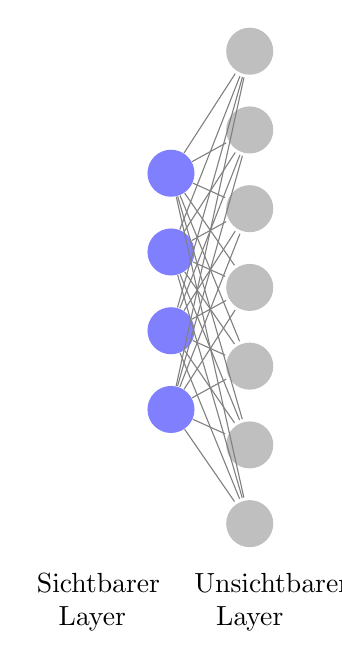
\begin{tikzpicture}[shorten >=1pt,-,draw=black!50, node distance=\layersep]
    \tikzstyle{every pin edge}=[<-,shorten <=1pt]
    \tikzstyle{neuron}=[circle,fill=black!25,minimum size=17pt,inner sep=0pt]
    \tikzstyle{visible neuron}=[neuron, fill=blue!50];
    \tikzstyle{hidden neuron}=[neuron, fill=gray!50];
    \tikzstyle{annot} = [text width=4em, text centered]

    % Draw the input layer nodes
    \foreach \name / \y in {1,...,4}
    % This is the same as writing \foreach \name / \y in {1/1,2/2,3/3,4/4}
        \node[visible neuron] (V-\name) at (0,-\y) {};
    
    % Draw the hidden layer nodes
    \foreach \name / \y in {1,...,7}
        \path[yshift=1.55cm]
        node[hidden neuron] (H-0-\name) at (\biglayersep,-\y cm) {};
        
    % Connect every node in the input layer with every node in the
    % hidden layer.
    \foreach \source in {1,...,4}
        \foreach \dest in {1,...,7}
            \path (V-\source) edge (H-0-\dest);

    % Annotate the layers
    \node[annot,below of=H-0-7, node distance=1cm] (hl 0) {Unsichtbarer Layer};
    \node[annot,left of=hl 0, node distance=2cm] (vli) {Sichtbarer Layer};
    %\node[annot,below of=vli, node distance=0.7cm] {(inputs)};
    
\end{tikzpicture}
}
   }
  \hspace{0.1\textwidth}
  %%----start of second subfigure----
  \subfloat[QBM]{
   \label{fig:qbm} %% label for second subfigure
   \scalebox{0.8}{
   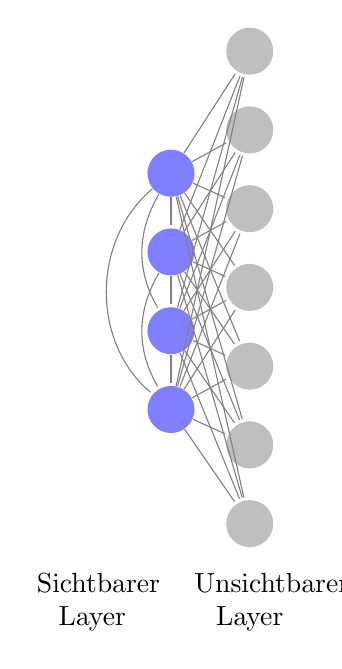
\begin{tikzpicture}[shorten >=1pt,-,draw=black!50, node distance=\layersep]
    \tikzstyle{every pin edge}=[<-,shorten <=1pt]
    \tikzstyle{neuron}=[circle,fill=black!25,minimum size=17pt,inner sep=0pt]
    \tikzstyle{visible neuron}=[neuron, fill=blue!50];
    \tikzstyle{hidden neuron}=[neuron, fill=gray!50];
    \tikzstyle{annot} = [text width=4em, text centered]

    % Draw the visible layer nodes
    \foreach \name / \y in {1,...,4}
    % This is the same as writing \foreach \name / \y in {1/1,2/2,3/3,4/4}
        \node[visible neuron] (V-\name) at (0,-\y) {};

    % Draw connections between visible nodes
    \path (V-1) edge (V-2);
    \path (V-1) edge [bend right = 30] (V-3);
    \path (V-1) edge [bend right = 50] (V-4);
    \path (V-2) edge (V-3);
    \path (V-2) edge [bend right = 30] (V-4);
    \path (V-3) edge (V-4);
    
    % Draw the hidden layer nodes
    \foreach \name / \y in {1,...,7}
        \path[yshift=1.55cm]
        node[hidden neuron] (H-0-\name) at (\biglayersep,-\y cm) {};
        
    % Connect every node in the visible layer with every node in the
    % hidden layer.
    \foreach \source in {1,...,4}
        \foreach \dest in {1,...,7}
            \path (V-\source) edge (H-0-\dest);

    % Annotate the layers
    \node[annot,below of=H-0-7, node distance=1cm] (hl 0) {Unsichtbarer Layer};
    \node[annot,left of=hl 0, node distance=2cm] (vli) {Sichtbarer Layer};
    %\node[annot,below of=vli, node distance=0.7cm] {(inputs)};
    
\end{tikzpicture}
}
   }\\[0pt] % horizontal break
 \caption[Schematische Architektur der verwendeten BMs]{Schematische Darstellung der Architekturen der in dieser Arbeit verwendeten BMs.}
 \label{fig:bms} %% label for entire figure
\end{figure}

\subsection{Quantum Boltzmann Machine}
\label{subsec:qbm}
Obwohl der im Abschnitt \ref{subsec:rbm} vorgestellte Trainings-Algorithmus der RBM effizient ausgeführt werden kann, unterliegt diese heuristische Vorgehensweise doch einigen Einschränkungen: Zum einen funktioniert diese Methode nur dann, wenn es keine Verbindungen innerhalb der Layer gibt. Die Kapazität der RBM, bestimmte Verteilungen der Daten anzunähern, ist im Vergleich zu der einer BM eingeschränkt. Zum anderen entspricht das in Gleichung \ref{eq:weight} genannte \\$\Delta weights\_momentum$, mit dem die Gewichte aktualisiert werden, nur grob dem Gradienten der \emph{Kullback-Leibler-Divergenz} (KL-Divergenz). Hierbei handelt es sich um das Maß für die Unterschiedlichkeit der Wahrscheinlichkeitsverteilungen der Trainingsdaten und der Konfigurationen der sichtbaren Neuronen im Modell. Dieses soll im Gradienten-Abstiegs-Verfahren minimiert werden, um die beiden Verteilungen einander anzugleichen. Der Gradient hat dabei die Form:
\begin{equation} \label{eq:kl-gradient}
\frac{\partial KL-Divergenz}{\partial w_{ij}} = \langle s_i s_j \rangle_{clamped} - \langle s_i s_j \rangle{unclamped}
\end{equation}
$s_i, s_j \in \{v, h\}$ sind hierbei die Neuronen, die sich an den Enden der zum Gewicht $w_{ij}$ zugehörigen Verbindung befinden. $\langle ... \rangle$ bezeichnet den Erwartungswert bzw. die durchschnittliche Wahrscheinlichkeit, dass beide Neuronen den Wert 1 besitzen. Dabei gibt \emph{clamped} an, dass die Konfiguration der sichtbaren Neuronen auf einen Datenpunkt festgelegt wird, während sie bei \emph{unclamped} unabhängig von möglichen Eingabedaten selbstständig vom Modell festgelegt wird \footnote{Zur Herleitung der Formel, vergleiche die Arbeit von Ackley et al. \cite{ackley1985learning}, insbesondere den Anhang.}. Letzteres geschieht jedoch bei der RBM nicht in dieser Reinform, da auch die in Gleichung \ref{eq:neg_ass} beschriebenen \emph{negative\_associations} indirekt von der Eingabe abhängen. Somit würde eine uneingeschränkte BM, die auch direkt aus dem Modell sampeln kann, die Minimierung der KL-Divergenz genauer ausführen. Dies könnte potentiell zu besseren Lernergebnissen führen.~\cite{hinton2012practical, ackley1985learning, Adachi15}

Gerade das klassische Sampeln aus dem Modell bedeutet einen sehr hohen Zeitaufwand. Insbesondere bei beliebiger Konnektivität des Modells ist das nur dann möglich, wenn für jedes Sampel iterativ die Werte der einzelnen Neuronen abhängig von den Werten ihrer benachbarten Neuronen berechnet werden. Dies wird solange wiederholt, bis sich ein Gleichgewicht einstellt, was meist aufgrund der langen Laufzeit nicht praktikabel ist.~\cite{Amin18, ackley1985learning, Adachi15}

Abhilfe schafft hier der Einsatz von QA. Wie in Abschnitt \ref{subsec:basics-qc} erwähnt, basieren die Berechnungen eines Quantum Annealers ebenfalls auf einer Energiefunktion. Mit der höchsten Wahrscheinlichkeit wird das Argument zurückgegeben, welches die Energiefunktion minimiert. In der Praxis werden mit niedrigerer Wahrscheinlichkeit zusätzlich andere Werte zurückgegeben. Die Wahrscheinlichkeitsverteilung der Rückgaben entspricht dabei approximativ einer Boltzmann-Verteilung. Weiterhin hat die Energiefunktion eines Quantum Annealers eine sehr ähnliche Form wie Gleichung \ref{eq:energiefunktion}. Die \emph{Quadratic Unconstrained Binary Optimization} (QUBO)-Formulierung, die zum Erstellen des erwünschten finalen Hamiltonians verwendet wird, hat die Form:
\begin{equation} \label{eq:qubo}
	Q(s_1, ..., s_n) = \sum_{ij}(J_{ij} s_i s_j) + \sum_i(b_i s_i)
\end{equation}
Die Variablen $s_i$ können hierbei ebenfalls die Werte 0 und 1 annehmen. Dadurch lässt sich die Energiefunktion einer BM als \emph{QUBO} darstellen. Durch Skalierung mit einem Parameter $\beta_{\text{eff}}$ lassen sich störende Einflüsse von Hardware-Eigenschaften wie fluktuierende Temperaturen, Noise, etc. korrigieren\footnote{Da diese Eigenschaften von der übergebenen Funktion abhängen können, stellt das sinnvolle Setzen dieses Parameters eine Herausforderung da \cite{Amin15, Korenkevych16, Adachi15, Benedetti16, Benedetti17}}.~\cite{Amin18, venegas2018cross, Adachi15, Benedetti16, Benedetti17} \\
Nun kann der Quantum Annealer für das Sampling zur Berechnung der beiden Erwartungswerte in Gleichung \ref{eq:kl-gradient} verwendet werden, wobei für ein Sampel jeweils ein Annealingaufruf ausreicht. Somit ist hier ein Quantenvorteil in Form eines Speedups zu erwarten. Die restlichen Teile des Trainings-Algorithmus der Quantum Boltzmann Maschine (QBM) werden weiterhin klassisch berechnet. Es handelt sich also um einen hybriden Algorithmus. Zu finden ist dieser Algorithmus als Pseudo-Code in Listing \ref{lst:qbm-algo}.~\cite{Amin18}\\

\lstinputlisting[caption={Trainings-Algorithmus einer Quantum Boltzmann Machine als Pseudo-Code.}, captionpos=b, abovecaptionskip=3pt, label={lst:qbm-algo}]{file.pseudo}

\noindent Experimente von Amin et al. \cite{Amin18} zeigen, dass dieser Algorithmus es ermöglicht, bessere KL-Divergenzen zu erreichen als vergleichbare klassische Varianten. Dies deutet auf einen weiteren Quantenvorteil hin. Eine der dafür verwendeten Architekturen, die semi-restricted QBM, wurde für diese Arbeit in angepasster Form übernommen \cite{Amin18}. Die verwendete Architektur ist in Abbildung \ref{fig:qbm} zu sehen.

\subsection{Anomalieerkennung mit Boltzmann Machines}
\label{subsec:anomaly-detec-bm}
Nun sollen die erwähnten Boltzmann Machine verwendet werden, um in einem Datensatz Anomalien zu erkennen. 
Das automatisierte Erkennen dieser Anomalien soll unsupervised erfolgen. Funktioniert eine BM, ordnet sie Anomalien basierend auf der gelernten Wahrscheinlichkeitsverteilung höhere Energien als den restlichen Datenpunkten zu, da diese mit einer geringeren Wahrscheinlichkeit auftreten. Zur Unterscheidung dieser Energieniveaus kann in der Testphase des Modells ein Schwellenwert dienen. Nur Punkte oberhalb des Schwellenwerts werden als Anomalien klassifiziert. Berechnet wird dieser Schwellenwert als empirisches $p$-Quantil des Trainingsdatensatzes, wobei in dieser Arbeit der in der Literatur verwendete Wert $p = 95\%$ gewählt wurde. Der Schwellenwert wird also so gewählt, dass ein Anteil $p$ (hier $95\%$) der Datenpunkte des Trainingsdatensatzes niedrigere Energien hat, während nur $(1 - p)$ (hier $5\%$) der Datenpunkte höhere Energiewerte haben. Dabei ist $p$ ein Hyperparameter der Anomalieerkennung, den man optimieren kann: Wird dieser Wert zu hoch gewählt, werden Anomalien nicht als solche identifiziert, ist er jedoch zu niedrig, so werden auch andere Datenpunkte fälschlicherweise als Anomalien eingestuft. Dabei ist im Zweifelsfall davon auszugehen, dass der zweitgenannte Fall vor dem Ersten zu bevorzugen ist. Nur eine erfolgreiche Anomalieerkennung rechtfertigt den Aufwand für ein entsprechendes Verfahren.~\cite{do2018energy, zhai2016deep}

\section{Evaluation} 
\label{sec:evaluation}

Die in Abschnitt \ref{sec:concept} erläuterten Konzepte wurden implementiert und anhand des multidimensionalen Datensatzes in
Abbildung \ref{fig:dataset} evaluiert.

\begin{figure}[h!]
    \centering
    \includegraphics[scale=0.3]{images/l_o7_c5_d3_p200_v1.pdf}
    \caption{3D-Datensatz mit 5 Clustern und 7 Anomalien}
    \label{fig:dataset}
\end{figure}

\noindent Dieses verfügt über vier Dimensionen, von denen jedoch nur die ersten drei tatsächliche Daten sind. Die vierte Dimension
enthält Informationen darüber ob ein Punkt eine Anomalie darstellt. Diese Information wird nicht zum Lernen genutzt, sondern
existiert nur, um das Datensatz zu visualisieren und eine Bewertung der Modelle nach Abschluss des Lernvorgangs zu ermöglichen.
Auf der Diagonalen ist die Wahrscheinlichkeitsverteilung der Daten gegeben.
Abseits der Diagonalen sind Dimensionen paarweise gegeneinander aufgetragen.

Der Datensatz enthält 1007 Punkte, sieben dieser Punkte sind Anomalien. Jede der ersten drei Dimensionen kann ganzzahlige
Werte im Intervall $[0,127]$ annehmen. Es werden also pro Dimension sieben Bit benötigt, das bedeutet um einen Punkt als
Eingabe für den Quantum Annealer darzustellen werden 21 Bit und damit auch 21 sichtbare Neuronen benötigt.

Der Datensatz wird halbiert, um das Modell mit unterschiedlichen Daten zu trainieren bzw. evaluieren.
Abschnitt \ref{subsec:hyperparameter} verschafft einen Überblick über die Hyperparameter der Modelle. Metriken, anhand welcher
die Leistung der Modelle bewertet wurden, sind in Abschnitt \ref{subsec:metriken} erläutert. Resultate der Hyperparameteroptimierung
durch einen Simulator werden in Abschnitt \ref{subsec:simulation} präsentiert. Schließlich werden in Abschnitt \ref{subsec:hardware} die
Ergebnisse der Ausführung auf Quantum Hardware, Simulator und der RBM verglichen.

\subsection{Hyperparameter}
\label{subsec:hyperparameter}
Da die BM selbst ein ML Modell ist, verfügt sie über mehrere Hyperparameter, welche entsprechend schrittweise optimiert werden müssen.
Um eine solche Optimierung sinnvoll zu gestalten wurde in der Implementierung darauf geachtet, einen einheitlichen Seed zu wählen, um reproduzierbare 
Initialisierung von Gewichten sicherzustellen. Die folgenden Hyperparameter wurden in der Implementierung verwendet und sind nach ihrer Relevanz sortiert:

\begin{description}
    \item[Anzahl Unsichtbarer Neuronen] ist der wichtigste Hyperparameter. Jedes unsichtbare
    Neuron muss durch ein logisches Qubit dargestellt werden und nimmt dadurch direkt
    Einfluss darauf, auf welcher Hardware das Modell in welchem Umfang ausgeführt
    werden kann.
    
    \item[Anzahl Epochen] gibt an, wie oft das Lernen auf dem Trainingsdatensatz wiederholt
    wird. Sie beeinflusst direkt die benötigte Rechenzeit.
    
    \item[Größe der Batches] reguliert in wie viele und wie große Trainingsschritte eine
    Epoche aufgeteilt wird. Während dies die Rechenzeit nicht beeinflusst, hat es
    signifikante Auswirkungen auf die schlussendliche Performanz.
    
    \item[Lernrate] bestimmt, wie viel pro Trainingsschritt gelernt wird.
    
    \item[Quantil] definiert, bei welcher Grenze der Schwellenwert gezogen werden sollte.
\end{description}

\noindent Im Rahmen dieser Arbeit wurden die drei wichtigsten Hyperparameter optimiert.
Um die Konfiguration der Hyperparameter und die damit einhergehende Qualität der Modelle zu
bewerten, wurden verschiedene Metriken verwendet. 

\subsection{Verwendete Metriken}
\label{subsec:metriken}
Zur Evaluierung der Ansätze wurden \emph{Recall}, \emph{Precision} und \emph{F1-Wert} benutzt.
Jede dieser Metriken liegt im Intervall $[0,1]$.\cite{tharwat2020classification}

\begin{description}
    \item[Der Recall] gibt an, wie viele Anomalien gefunden werden
        konnten. Gerade in sicherheitskritischen Anwendungen ist ein hoher Recall sehr wichtig.
        Er ist jedoch nicht ausreichend, da er seinen Maximalwert immer annimmt, wenn das
        Modell sämtliche Instanzen als Anomalien einstuft.

    \item[Die Precision] gibt an, wie viele der 
        der gefundenen Anomalien auch wirklich welche sind. Das hier vorliegende Problem ist,
        dass sie genau dann maximal wird, wenn alle gefundenen Instanzen
        richtig klassifiziert wurden. Das bedeutet, wenn das Modell keine Anomalien
        findet, ist die Precision trotzdem maximal, der Recall wird jedoch massiv sinken.

    \item[Der F1-Wert] ist das harmonische Mittel aus Recall und Precision.
        Das heißt, er wird nur maximal, wenn seine beiden Bestandteile ihr Maximum annehmen.
        Da keine der beiden anderen Metriken alleine ausreichend ist, benutzen wir den F1-Wert
        für die weitere Evaluation.
\end{description}
 

\subsection{Resultate der Simulation}
\label{subsec:simulation}

Aufgrund limitierter Rechenzeit für Quantum Computer, wurde die Hyperparameteroptimierung
mithilfe von Simulated Annealing (SA) auf einem klassischen Rechner durchgeführt. Verwendet wurden 
dabei ein Intel I7 8700 mit Ubuntu 20.04 und Python 3.8.\\\\
Um Berechnungen auf einem Quantum Annealer durchführen zu können, wird ein \emph{Embedding} benötigt. Ein
solches wird in Abhängigkeit der benötigten logischen Qubits\footnote{theoretisch fehlerfreie Qubits mit beliebiger Konnektivität. Diese müssen im Embedding-Prozess aufgrund der eingeschränkten Konnektivität der physikalischen Qubits der verwendeten Hardware abgebildet werden.} 
berechnet. Wie bereits in \ref{subsec:hyperparameter} erwähnt, ist die Anzahl der unsichtbaren Neuronen hierbei sehr 
wichtig, da diese variabel ist und die Anzahl der benötigten logischen Qubits direkt
beeinflusst. Für unseren Datensatz konnte auf dem
\emph{D-Wave 2000Q} ein Embedding für bis zu 94 unsichtbare Neuronen gefunden werden, auf dem
\emph{Advantage} für bis zu 632 unsichtbare Neuronen \cite{quantum_hardware}. Abbildung \ref{fig:hidden_units} zeigt
den erreichten F1-Wert für die jeweilige Anzahl an unsichtbaren Neuronen. Aufgetragen 
sind Quantensimulation und klassischer Ansatz.
\begin{figure}[h!]
    \centering
    \includegraphics[scale=0.6]{images/hidden_figure.pdf}
    \caption{F1-Werte für ansteigende Anzahl unsichtbarer Neuronen}
    \label{fig:hidden_units}
\end{figure}\\\\
Die Abbildung \ref{fig:hidden_units} veranschaulicht, dass der Simulator für seinen optimalen F1-Wert deutlich weniger 
unsichtbare Neuronen benötigt. Das Optimum des Simulators liegt bei 82 Neuronen mit einem F1-Wert von $0,35$, während die RBM 
ihren optimalen F1-Wert von $0,33$ erst bei 157 Neuronen erreicht.
Die QBM erreicht also mit weniger Ressourcen ein besseres Ergebnis.
\begin{figure}[h!]
    \centering
    \includegraphics[scale=0.6]{images/epoch_figure.pdf}
    \caption{F1-Werte für ansteigende Anzahl an Epochen}
    \label{fig:epochs}
\end{figure}\\\\
Anschließend wurde die Anzahl an Epochen optimiert. Dafür wurde jeder Ansatz mit seinem
Optimum an unsichtbaren Neuronen mehrfach ausgeführt. Abbildung \ref{fig:epochs} trägt
wieder den Vergleich zwischen klassischem Ansatz und Quantensimulation auf.
Es ist klar erkennbar, dass die Simulation den klassischen Ansatz übertrifft.
Während der klassische Ansatz sein Optimum bei 13 Epochen erreicht und dabei einen F1-Wert
von $0,33$ besitzt, ist das Optimum der Simulation bei 14 bzw. 16 Epochen mit einem F1-Wert von
$0,375$. Der Simulator erreicht also insgesamt einen höheren F1-Wert als der klassische
Ansatz. Außerdem liefert die Simulation bei wenigen Epochen konstant bessere
Ergebnisse als der klassische Ansatz. Bei sieben
Epochen liegt der F1-Wert bereits bei $0,35$, übertrifft also das globale
Optimum des klassischen Ansatzes und ist auch beinahe am globalen Optimum der
Simulation. Im Vergleich zum globalen Optimum wird hier aber nur die halbe Rechenzeit benötigt.
Aufgrund der geringen verfügbaren Rechenzeit auf Quantum Hardware
wurde die 7 als Optimum für Epochen und weitere Optimierungsschritte angenommen,
während für den klassischen Ansatz die 13 ausgewählt wurde.
\begin{figure}[h!]
    \centering
    \includegraphics[scale=0.6]{images/batchsize_figure.pdf}
    \caption{F1-Werte für ansteigende Batchgrößen}
    \label{fig:batchsize}
\end{figure}\\\\
Abbildung \ref{fig:batchsize} zeigt, dass sowohl der klassische Ansatz als auch die
Simulation ihr Optimum bei einer Batchgröße von zehn erreichen. 
Der klassische Ansatz verbleibt dabei auf einem F1-Wert von $0,33$, während der
Simulator bei $0,35$ verbleibt.

\subsection{Resultate auf Quantum Hardware}
\label{subsec:hardware}

Das Modell wurde auf Quantum Hardware mit den im Simulator optimierten Hyperparametern ausgeführt.
Zur Verfügung standen dabei der D-Wave 2000Q, der Advantage und der Fujitsu DAU.
Die Tabelle \ref{fig:hardware_comparison} zeigt die gemessenen Ergebnisse der jeweiligen
Ausführung.
\begin{table}[h!]
    \centering
    \begin{tabular}{l | c | c | c | c | c}
     & RBM & Simulator & D-Wave 2000Q & Advantage & Fujitsu DAU \\
      \hline
     F1-Score           & 0.33 &   0.35 &     0.14 &  0.21 & 0  \\
     Recall             &1    &      1 &     0.67 &  0.67 & 0  \\ 
     Precision          &0.2  &   0.21 &    0.076 & 0.125 & 0  \\ 
     QPU Time [s]       &-    &  85.73 &    126.7 & 150.54 & 99.18  \\ 
\end{tabular}
    \caption{Vergleich der Ausführungen anhand verschiedener Metriken}
    \label{fig:hardware_comparison}
\end{table}\\\\
Während keiner der Quantum Computer die gleiche Performanz wie der Simulator bieten konnte,
sind die Ergebnisse weit vom Zufall entfernt. Beide D-Wave Rechner konnten im Gegensatz zum Simulator eine Anomalie nicht
finden und haben somit einen identischen Recall. Der Advantage hat eine um $62,3 \%$ höhere Precision. Das bedeutet,
dass weniger Clusterpunkte als Anomalien identifiziert wurden. Der bessere F1-Wert spiegelt dies ebenfalls wieder.
\begin{figure}[h!]
    \centering
    \includegraphics[scale=0.6]{images/Advantage_DWave_SA_RBM_energies_multiple.pdf}
    \caption{Normalisierte Energien von Anomalien und Clusterpunkten für verschiedene Ansätze. Die blaue Linie ist der Energie-Schwellenwert.}
    \label{fig:Energies}
\end{figure}\\\\
In Abbildung \ref{fig:Energies} ist eine kompakte Übersicht zum Vergleich der Ergebnisse als Box-Plot gegeben. Aufgetragen sind die Energieniveaus der Clusterpunkte bzw. Anomalien des Testdatensatzes für die Systeme Advantage, D-Wave 2000Q, Simulator und RBM. Zu sehen sind außerdem die durch das Quantil gegebenen respektiven Schwellenwerte, die aus dem Trainingsdatensatz erlernt wurden. Um die Werte optisch besser in Vergleich zu setzen wurden sie hier normalisiert. Dies ist möglich, da für die Klassifizierung der Anomalien nur der Unterschied der Energieniveaus ausschlaggebend ist.

\section{Fazit} 
\label{sec:conclusion}

Wie die Ergebnisse in Abschnitt \ref{subsec:simulation} zeigen, scheinen die in Kapitel \ref{sec:related} und Abschnitt \ref{subsec:qbm} vermuteten Quantenvorteile in Form eines beschleunigten Lernvorgangs und einer
verbesserten Leistungsfähigkeit laut Simulator vorhanden zu sein. Weiterhin zeigen die Ergebnisse, dass das neuere System Advantage bei der selben Wahl an Hyperparametern eine erheblich bessere Performanz als sein
Vorgänger D-Wave 2000Q erzielt. Es ist zu hoffen, dass sich die Quantum Computer zukünftig weiter verbessern werden und sich der Leistung des Simulators annähern oder diesen sogar übertreffen werden. 
Der von uns implementierte Ansatz ist aufgrund seiner kompakten Struktur von nur zwei Layern sehr flexibel. Jeder Layer kann in der Anzahl seiner Neuronen frei angepasst werden. Dies ermöglicht ein Skalieren auf eine
beliebige Anzahl an Qubits, wodurch hochdimensionale Datensätze verarbeitet werden können. Da die Datenpunkte zudem sequentiell vom Annealer bearbeitet werden, schränkt die Anzahl an verfügbaren Qubits nicht die Größe des
Trainings- bzw. Testdatensatzes ein.\\\\
Da Quantenvorteile zu bestehen scheinen, bedarf es weiterer Untersuchungen. Als erster Schritt muss eine umfassendere und sorgfältigere Hyperparameteroptimierung auf den jeweiligen Plattformen durchgeführt werden, um
sicherzustellen, dass die jeweiligen Optima auch tatsächlich gefunden werden.

Sollten diese Quantenvorteile nach genauer Betrachtung noch immer bestehen, so muss ihr Ursprung ermittelt werden. Hierzu könnte z.B. der Einfluss der in Abschnitt \ref{subsec:qbm} erwähnten Verbindungen innerhalb der Layer untersucht werden.
